\title{The Geometry of the Monodromy Theorem\footnote{This article has been conceived during the stay of the author at the Mathematics Institute of the Vietnam Institute for Sciences at Hanoi and has been informally lectured at the Kyoto Sympostium on Algebraic Geometry in January 1977.}}\label{art15}
\markright{The Geometry of the Monodromy Theorem}


\author{By~ L$\hat{\rm e}$ D$\tilde{\rm u}$ng Tr\'ang}
\markboth{L$\hat{\rm e}$ D$\tilde{\rm u}$ng Tr\'ang}{The Geometry of the Monodromy Theorem}

\date{}
\maketitle{}

\setcounter{page}{191}

{\bf Introduction.}
\setcounter{pageoriginal}{156} Let\pageoriginale $(X,x)$ be the germ of an analytic space and $f:(X,x) \to (\bfC, 0)$ be the germ of an analytic function. We shall still denote $X$ and $f$ representants of the corresponding germs. Let us suppose $X \subset U \subset \bfC^N$ where $U$ is an open subset of $\bfC^N$ and $X$ is closed in $U$.

Let us suppose that for any $t \neq 0$ sufficiently small, $f = t$ is smooth.  It has been proved in \cite{art15-key3} or \cite{art15-key6} that if $\epsilon > 0$ is small enough and $0< \eta \ll \epsilon$, we have a smooth (i.e. $C^\infty$) fibration:
$$
\varphi_{\epsilon, \eta}: B_\epsilon \cap f^{-1} (D^*_\eta) \to D^*_\eta
$$
induced by $f$, where $B_\epsilon$ is the closed ball of $\bfC^N$ centered at $x$ with radius $\epsilon>0$ and $D^*_\eta = \{z \in\bfC |0< |z| \leqslant \eta\}$. We shall call this fibration the Milnor fibration of $f$ at $x$ (cf. \cite{art15-key11}  when $X = \bfC^N$). 


The monodromy of this fibration is called the local monodromy of $f$ at $x$ (cf. \cite{art15-key6}). We prove under the preceding hypothesis:

\begin{theorem*}{\rm (the Monodromy Theorem):} The local monodromy of $f$ at $x$ is quasi-unipotent, i.e. its eigenvalues are roots of unity.
\end{theorem*}

In \cite{art15-key1} this theorem has been proved using the resolution of singularities. In \cite{art15-key2}, A. Grothendieck has given a proof which applies in the case we have a proper mapping $f: X \to C$; this proof actually uses the resolution of singularities and applies in any characteristic when there is a resolution of singularities. Another proof with a topological flavour, but still using the resolution of singularities is given by A. Landman in \cite{art15-key5}.

In this paper we are giving a topological proof of the monodromy theorem which does not use the resolution of singularities and which gives\pageoriginale a topological interpretation to the eigenvalues. The proof uses the notion of relative monodromy (cf. \cite{art15-key6}) which is an avatar of the Lefschetz method for the study of the monodromy. Its strong interest comes from the use of a precise geometric description of the singularity. This leads to an interesting filtration of the Milnor fiber of $f$ at $x$.

I thank N. A'Campo for noticing a mistake in the original paper concerning the hypersurfaces. I thank K. Saito to have helped me to settle down correctly the proof. I thank R. Thom for the constant interest he showed in this paper.

\section{Basic facts about the relative monodromy}\label{art15-sec1}
Now we recall some results about the relative monodromy. cf. \cite{art15-key6}. We still use the notations defined in the introduction. Let $z_1$ be a linear form of $\bfC^N$, say the first coordinate of $\bfC^N$. The restriction of $z_1$ to $X$ and $f$ defines a mapping $(z_1, f)$ of $X$ into $\bfC^2$. From \cite{art15-key7} and \cite{art15-key6}, because $X-f^{-1}(0)$ is smooth, we have the following theorem:

\begin{thm}\label{art15-thm1.1}
Suppose that $z_1 =0$ be sufficiently general, then we have polydiscs $D \times P \subset \bfC^N$ centered at $x$ and $D \times D'\subset \bfC^2$ centered at $(z_1 (x), 0)$, a curve $\Gamma \subset (D \times P) \cap X$ and a curve $\Delta \subset D \times D'$  such that:
\begin{itemize}
\item[\rm (1)] the restriction $\Phi$ of $(z_1,f)$ to $(D \times P) \cap X$ is critical along $\Gamma$ outside $f^{-1} (0)$, moreover it induces a smooth fibration of $\Phi^{-1} (D \times D' - \Delta)$ onto $D \times D' - \Delta$;

\item[\rm (2)] $f$ induces a smooth fibration $\Phi^{-1} (D \times D' - D \times \{0\})$ onto $D' -\{0\}$ which is fiber isomorphic to the Milnor fibration of $f$  at $x$;

\item[\rm (3)] $f$ induces a smooth fibration of $(\{0\} \times P) \cap \Phi^{-1} (D \times D' - \{0\})$ onto $D'-\{0\}$ which is fiber isomorphic to the Milnor fibration of the restriction of $f$ to $X \cap \{z_1 = 0\}$ at $x$;

\item[\rm (4)]  for any $x \in \Delta - \{0\}$ the fibers $\Phi^{-1} (x)$ have only one quadratic ordinary singular point at $y = \Gamma \cap \Phi^{-1} (x)$.
\end{itemize}
\end{thm}

In \cite{art15-key8} and \cite{art15-key6} we have called $\Gamma$ the polar curve of $f$ relatively to $z_1 = 0$ and $\Phi (\Gamma) = \Delta_0$ its Cerf diagram. Notice that it may happen that $\Delta = \Delta_0$, but in general $\Delta = \Delta_0 \cup (D \times \{0\})$.

In \cite{art15-key6}\pageoriginale we have seen that in this situation we have defined a smooth mapping $h$ of the Milnor fiber $\Phi(D \times \{\eta\})$ onto itself where $\eta \in\partial D'$ which is a characteristic diffeomorphism of Milnor fibration of $f$ at $x$. Moreover $h$ lifts a  diffeomorphism $\Psi$ of $D \times \{\eta\}$ onto itself such that the following diagram is commutative:
\[
\vcenter{
\xymatrix{
\Phi^{-1} (D \times \{\eta\}) \ar[r]^{h} \ar[d]_\varphi & \Phi^{-1} (D \times \{\eta\}) \ar[d]^{\varphi}\\
D \times \{\eta\} \ar[r]^{\Psi} & D \times \{\eta\}
}} \tag{1.2}\label{art15-eq1.2}
\]
where $\varphi$ is induced by $\Phi$ and $\Psi$ satisfies the following properties:
\begin{itemize}
\item[(1)] $\Psi(0,\eta) = (0,\eta)$

\item[(2)] $\Psi (D \times \{\eta\}) \cap \Delta = (D \times \{\eta\}) \cap \Delta$.
\end{itemize}
Further properties of $\Psi$ will be given in the next paragraph. In \cite{art15-key6} it has been seen that $h$ induces a smooth mapping of $\Phi^{-1}(0,\eta)$ onto itself which is a characteristic diffeomorphism of the Milnor fibration of the restriction of $f$ to $X \cap \{z_1 = 0\}$. Then $h$ induces an automorphism of $H_* (\Phi^{-1} (D \times \{\eta\}), \Phi^{-1} ((0,\eta)))$ which defines the relative local monodromy of $f$ at $x$. From the fact that $X - f^{-1} (0)$ is smooth and the (4) of the Theorem (\ref{art15-thm1.1}) cited above, a reasoning as in \cite{art15-key8} leads to:

\setcounter{lemma}{2}
\begin{lemma}\label{art15-lem1.3}
$H_k (\Phi^{-1} (D \times \{\eta\}), \Phi^{-1} ((0,\eta))) =
\left\{  \begin{aligned}
0 \text{ if } k \neq \dim_C f^{-1} (t)\\
\bfZ^r \text{ if } k = \dim_C f^{-1}(t)
  \end{aligned} \right.$
with $t$ small enough and $t \neq 0$, and $r$ equal to the number of points of $\Delta \cap (D \times \{\eta\})$ or $\Gamma \cap \Phi^{-1} (D \times \{\eta\})$.
\end{lemma}

Notice that $\Gamma$ may be $\oslash$ and thus $H_* (\Phi^{-1} (D \times \{\eta\}), \Phi^{-1} ((0,\eta)))$ may entirely vanish. 

Now we are going to give a more precise description of $\Psi$ which will allow use to prove the monodromy theorem.

\section{The Carrousel}\label{art15-sec2}
We are\pageoriginale going to recall the results of \cite{art15-key6} and \cite{art15-key7} which describe $\Psi$.

Let 
\begin{equation*}
\left\{
\begin{aligned}
\lambda  & = t^r \\
z_1 & = \sum\limits_{j \geqslant r_i} a_{ij} t^j \quad a_{ir_i} \neq 0 
\end{aligned}
\right.
\tag{2.1}\label{art15-eq2.1}
\end{equation*}
be a parametrization of $\Delta_i$.

Let us index the $\Delta_1$, $i=1, \ldots, k$, such that  for any $1 \leqslant i \leqslant i_1 - 1$, we have
\begin{align*}
& \left\{
\begin{aligned}
& \frac{r_1}{r} = \frac{r_i}{r} = \frac{m'_1}{n'_1} \text{ with } (m'_1, n'_1) =1 \\
& a_{1r_1} = a_{ir_i} = \alpha_1
\end{aligned}
\right. \tag{2.2}\label{art15-eq2.2}\\
& \qquad \ldots \ldots \ldots \ldots 
\end{align*}
for any $i_l \leqslant i \leqslant i_{l+1} - 1 =k$, we have 
\begin{equation*}
\left\{
\begin{aligned}
& \frac{r_{i_l}}{r} = \frac{r_i}{r} = \frac{m'_l}{n'_l} \text{ with } (m'_l, n'_l) = 1\\
& a_{i_l r_{i_l}} = a_{ir_i} =\alpha_l
\end{aligned}
\right.
\end{equation*}
and moreover
$$
\frac{m'_1}{n'_1} \geqslant \frac{m'_2}{n'_2} \geqslant \cdots \geqslant \frac{m'_l}{n'_1}
$$
all couples $\left(\dfrac{m'_1}{n'_1}, \alpha_i \right)$ are distinct and if $\dfrac{m'_j}{n'_j} = \dfrac{m'_{j+1}}{n'_{j+1}}$, we have $|\alpha_{j}|\leqslant |\alpha_{j+1}|$. 

Let us call $C_1, \ldots, C_l$ the curves defined by 
\begin{equation*}
\left\{
\begin{aligned}
\lambda & = t^{n'j} \\
z_1 & = \alpha_j t^{m'j}
\end{aligned}
\right.
\qquad j = 1, \ldots, l. \tag{2.3}\label{art15-eq2.3}
\end{equation*}

If $\eta$ is small enough, it is clear that the points of $(D \times \{\eta\}) \cap (\Delta_{i_j} \cup \ldots \cup \Delta_{i_{j+1}-1})$ lie in a neighbourhood of $(D\times \{\eta\}) \cap C_j$. More precisely

\setcounter{lemma}{3}
\begin{lemma}\label{art15-lem2.4}
If $\eta$\pageoriginale is small enough, in $D \times \{\eta\}$ there are disjoint discs $\delta_{j\mu} (j = 1, \ldots, l$ and $\mu = 1, \ldots, n'_j)$ centered at the $n'_j$ points of $(D \times \{\eta\}) \cap C_j$, when $j = 1, \ldots, l$, such that 
$$
(D \times \{ \eta\}) \cap (\Delta_{i_j} \cup \ldots \cup \Delta_{i_{j+1} -1}) \subset \bigcup\limits^{n'_j}_{\mu = 1} \delta_{j\mu}.
$$
Moreover the number of points of $\delta_{j\mu} \cap (\Delta_{ij} \cup \ldots \cup \Delta_{i_{j+1}-1})$  is the same for $\mu=1, \ldots, n'_j$ and the $\delta_{j\mu}$ have the same radius for $\mu =1,\ldots, n'_j$.
\end{lemma}

Now let us suppose that:
\begin{align*}
& \left|
\begin{aligned}
& \frac{m'_1}{n'_1}  = \ldots = \frac{m'_{j_1 -1}}{n'_{j_1 -1}}\\
&  \frac{m'_{j_1}}{n'_{j_1}}   = \ldots = \frac{m'_{j_2 -1}}{n'_{j_2 -1}}\\
& \ldots \ldots \ldots \\
& \frac{m'_{j_s}}{n'_{j_s}} = \ldots = \frac{m'_l}{n'_l}
\end{aligned}
\right. \tag{2.5}\label{art15-eq2.5}\\
\text{ and  } \hspace{3cm} & \frac{m'_1}{n'_1} > \frac{m'_{j_1}}{n'_{j_1}} > \ldots > \frac{m'_{j_s}}{n'_{j_s}}. \hspace{3cm}
\end{align*}

\setcounter{lemma}{5}
\begin{lemma}\label{art15-lem2.6}
If $\eta$ is small enough, in $D \times \{\eta\}$ there are closed discs centered at $(0,\eta)$, say $D_1 \subset D'_1 \subset \ldots \subset D'_{s-1} \subset D_s \subset D$ such that 
\begin{itemize}
\item[\rm 1)] the interior $\mathring{D}_1$ contains the $\delta_{j\mu}$ with $j=1, \ldots, j_1-1$ and $\mu=1,\ldots, n'_j$;

\item[\rm 2)] the open annulus $\mathring{D}_2 - D'_1$ contains the $\delta_{j\mu}$ with $j = j_1, \ldots, j_2 -1$ and $\mu =1, \ldots, n'_j$;

$\ldots \ldots \ldots \ldots $

\item[\rm s)] the open annulus $\mathring{D}_s - D'_{s-1}$ contains the $\delta_{j\mu}$ with $j = j_s, \ldots , l$ and $\mu = 1, \ldots, n'_j$.
\end{itemize}
\end{lemma}

Now we can summarize the properties of $\Psi$ (cf. \cite{art15-key6} and \cite{art15-key8}) as follows:

\setcounter{subsection}{6}
\subsection{}\label{art15-subsec2.7}
\begin{itemize}
\item[1)] $\Psi$ is a smooth diffeomorphism of $D \times \{\eta\}$ onto itself;

\item[2)] its restriction to $D_1 - \bigcup\limits^{j_1 -1}_{j=1} \bigcup\limits^{n'_j}_{\mu=1} \delta_{j\mu}$  is a rotation of angle $2\pi \dfrac{m'_1}{n'_1}$

$\ldots\ldots \ldots \ldots $\pageoriginale

its restriction to $(\mathring{D}_s - D'_{s-1}) - \bigcup\limits^l_{j=j_s} \bigcup\limits^{n'j}_{\mu=1} \delta_{j\mu}$ is a rotation of angle $2\pi \dfrac{m'_{js}}{n'_{js}}$;

\item[3)] its restriction to $\partial D \times \{\eta\}$ is the identity;

\item[4)] its restriction to each circle centered at $(0, \eta)$ and contained in $\mathring{D}_i - D'_{i-1}$ and $D - D_s$ is a rotation.
\end{itemize}

The we define a class of smooth diffeomorphisms of a disc $D$ onto itself to which $\Psi$ will belong.

\setcounter{lemma}{7}
\begin{definition}\label{art15-def2.8}
Any diffeomorphism of $D$ onto itself which maps the center of $D$ on itself, which has a fixed point $x \not\in \partial D$ and the restriction of which is the identity on $\partial D$ is called a carrousel with one distinguished point $x \in \mathring{D}$.
\end{definition}

\begin{definition}\label{art15-def2.9}
A roll is a diffeomorphism $\Psi$ of an open annulus $\mathring{D} - D'$ onto itself such that:
\begin{itemize}
\item[1)] there are circles $S_1, \ldots,S_m$ contained in $\mathring{D} - D'$ and discs $\delta_{ij} \subset \mathring{D} - D' (i=1,\ldots, m, j = 1, \ldots, q)$ centered at points $x_{ij}$ $(j = 1, \ldots,q)$ equidistributed on $S_i (i =1,\ldots, m)$ and of the same radius for any fixed $i$;

\item[2)] there are the same number of distinguished points in each $\delta_{ij}$ $(j=1,\ldots, q)$ for a given $i$, such that $\Psi$ maps $\delta_{ij}$ onto $\delta_{ij+1}$ for $j=1, \ldots, q^{-1}$ (resp. $\delta_{iq}$ onto $\delta_{i1}$) and the distinguished points of $\delta_{ij}$ onto those of $\delta_{ij+1}$ for $j = 1, \ldots, q^{-1}$ (resp. those of $\delta_{iq}$ onto those of $\delta_{i1}$);

\item[3)] the restriction of $\Psi$ to $\mathring{D} - D' - \bigcup\limits_{i,j} \delta_{ij}$ is a rotation of angle $2\pi \dfrac{p}{q}$, $(p,q) =1$.
\end{itemize}
\end{definition}

If $\Psi$ is a roll, $\Psi^q$ induces a diffeomorphism $\Psi_{ij}$ of $\delta_{ij}$ onto itself which maps the distinguished points of $\delta_{ij}$ onto themselves. We shall call the diffeomorphisms $\Psi_{ij}$ the {\em distinguished diffeomorphisms of the roll}.
\begin{figure}[H]
\centering
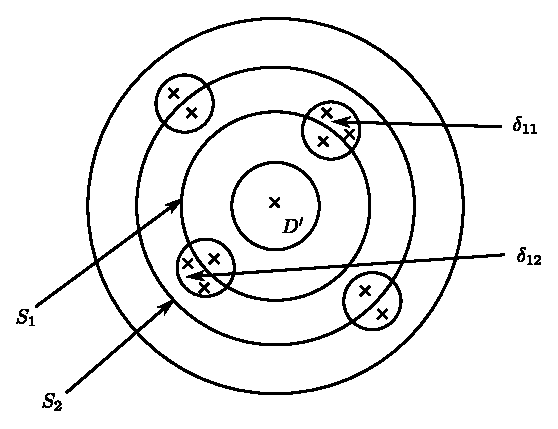
\includegraphics{fig15-1.eps}
\end{figure}\pageoriginale

We have defined a carrousel with one distinguished point, we suppose we have defined carrousels with $n'$ distinguished points, $1 \leqslant n' < n$, we define what is a carrousel with $n$ distinguished points.

\begin{definition}\label{art15-def2.10}
A `carrousel with $n$ distinguished points' is a diffeomorphism $\Psi$ of $D$ onto itself such that:
\begin{itemize}
\item[1)] there are discs $D_1 \subset D'_1 \subset D_2 \subset \ldots \subset D_k\subset D$ such that the restriction $\Psi_i$ of $\Psi$ to $\mathring{D}_i - D'_{i-1}$ is a roll;

\item[2)] the $n$ distinguished points of $\Psi$ are the distinguished points of the $\Psi_i$;

\item[3)] the distinguished diffeomorphisms of each roll are
\begin{itemize}
\item[a)] either carrousels with $n'$ distinguished with $1\leqslant n' < n$;

\item[b)] or $k=1$ and the roll $\Psi_1$ has only one distinguished diffeomorphism which satisfies 1) and 2); then if it satisfies 3)-b) this process will stop after $l$ steps with carrousels with $n'$ distinguished points with $1 \leqslant n' <n$. Such a carrousel is called a carrousel which simplifies after $l$ steps.
\end{itemize}
\end{itemize}
\end{definition}

\begin{example*}
(cf. \cite{art15-key6}\pageoriginale and \cite{art15-key7}).
\end{example*}

\setcounter{lemma}{10}
\begin{lemma}\label{art15-lem2.11}
The smooth mapping $\Psi: D \times \{\eta\} \to D \times \{ \eta\}$ of (\ref{art15-subsec2.7}) is actually a carrousel the distinguished points of which are $(\Delta_1 \cup \ldots \cup \Delta_k) \cap (D \times \{\eta\})$.
\begin{figure}[H]
\centering
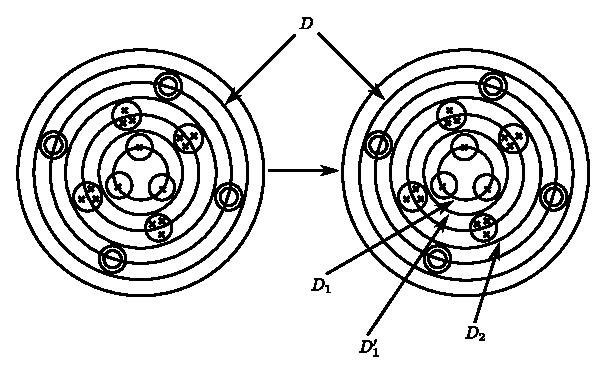
\includegraphics{fig15-2.eps}
\end{figure}
\end{lemma}

\section{The Monodromy Theorem:}\label{art15-sec3}
We can summarize the preceding results by 

\begin{thm}\label{art15-thm3.1}
$\eta > 0$ is small enough, there is a commutative diagram (cf. (\ref{art15-eq1.2})):
\[
\xymatrix{
\Phi^{-1} (D \times \{\eta\}) \ar[r]^{h} \ar[d] & \Phi^{-1} (D \times \{\eta\}) \ar[d]\\
D \times \{\eta\} \ar[r]^{\Psi} & D \times \{\eta\} 
}
\]
such that:
\begin{itemize}
\item[1)] $\Psi$ is a carrousel the distinguished points of which are $(D \times \{\eta\}) \cap \Delta$;

\item[2)] $h$ is\pageoriginale a characteristic diffeomorphism of the Milnor fibration of $f$ at $x$;

\item[3)] $h$ induces a diffeomorphism of $\Phi^{-1}(0,\eta)$ onto itself which is a characteristic diffeomorphism of the Milnor fibration of the restriction of $f$ to $X \cap \{z_1 = 0 \} $ at $x$;

\item[4)] the fibers of $\varphi$ over the distinguished points of $\Psi$ are singular and have only one ordinary quadratic singular point, the other fibers of $\varphi$ are smooth.
\end{itemize}
\end{thm}

Moreover, it is clear that if $\dim_\bfC f^{-1} (t) =0$ when $t \neq 0$ is small enough, the monodromy theorem is true.

(H) {\em Let us assume it is true when $1 \leqslant \dim_\bfC f^{-1} (t) < n$.}

Suppose now that $\dim_\bfC f^{-1} (t) =n$.

From the induction hypothesis we know that for any parametrization $\pi: (\bfC,0)  \to (\bfC^2, 0)$ of a germ of curve $(C,0)$ in $(\bfC^2,0)$, such that $(C,0)$ does not lie inside $(\bfC \times \{0\} 0)$ the monodromy of the pullback $f_\pi$ of $\Phi$ is quasi-unipotent:
\[
\xymatrix{
X_\pi, 0 \ar[r]\ar[d]^{f_\pi} & X,0\ar[d]^{\Phi} \\
(\bfC, 0) \ar[r]_\pi & (\bfC^2 , 0)
}
\]
Then we obtain:

\begin{lemma}\label{art15-lem3.2}
For any point $x \in D_i - (\mathring{D}'_{i-1} \bigcup\limits_{j,k} \delta_{ijk})$, $h^{n'_{ji}}$ induces an automorphism of $H_* (\Phi^{-1} (x))$ which is quasi-unipotent.
\end{lemma}

\begin{proof}
Consider a curve $C_x$ parametrized by
\begin{equation*}
\left\{
\begin{aligned}
\lambda & = t^{n'_{ji}}\\
z_0 & = \alpha (x) t^{m'_{ji}}
\end{aligned}
\right. \tag{*}
\end{equation*}
such that $x \in C_x$. It is clear that such a curve exists and does not contain any point of $\Delta \cap (D \times \{\eta \})$ as
$$
C_x \cap ( D \times \{\eta\}) = C_x \cap (D_i - (\mathring{D}'_{i-1} \bigcup\limits_{j,k} \delta_{ijk})).
$$

It\pageoriginale is enough now to notice that $\Psi$ induces a bijection of $C_x \cap (D \times \{\eta\})$ onto itself which is lifted in a characteristic diffeomorphism of the fibration $\Phi^{-1} (C_x \cap (D \times \partial D')) \to \partial D'$  induced  by $f$. Finally the monodromy of this fibration is quasi-unipotent as its pull back by (*) is quasi-unipotent according to the induction hypothesis.

Actually we have a more precise result which will allow us to prove the monodromy theorem by induction on the dimension of the fiber
\end{proof}

\begin{lemma}\label{art15-lem3.3}
Let $\Psi_{ijk} :\delta_{ijk}\to \delta_{ijk}$ a distinguished carrousel of the carrousel $\Psi$. Let $x$ be a point of $\delta_{ijk} \to \Delta$ on which the action of $\Psi_{ijk}$ is one of the rotations of this carrousel. Then there is a power $h^q$ of $h$ which induces a quasi-unipotent automorphism of $H_* (\Phi^{-1} (x))$. This property is true for the distinguished carrousels of $\Psi_{ijk}$ and so on.
\end{lemma}

Let $2 \pi p/q$ be the angle of the rotation induced by $\Psi_{ijk}$ on $x$. We may choose $q$ multiple of $n'_{j_i}$. The proof is the same as the one of (\ref{art15-lem3.2}) by considering a curve parametrized by
\begin{equation*}
\begin{cases}
\lambda = t^q\\
z_0 = \alpha_i t^{m'_j \frac{q}{n'_{j_i}}} + \beta (x) t^{m'_j \frac{q}{n'_{j_i}} + p} 
\end{cases}
\end{equation*}
which goes through $x$.

Because of the specific character of the points $x$ which appear in (\ref{art15-lem3.2}) and (\ref{art15-lem3.3}) we shall call the points of $D_i - (\mathring{D}'_{i-1} \bigcup\limits_{j,k} \delta_{ijk})$ the {\em rotating points} of the carrousel $\Psi$. The distinguished carrousels of distinguished carrousels of $\Psi$ and so on are called {\em successive distinguished carrousels of $\Psi$}. The rotating points of the successive distinguished carrousels of $\Psi$ are called the {\em rolling points} of $\Psi$.


Notice that if $\Psi$ is a carrousel with one distinguished point the centre of $D$ might be the only rolling point of $\Psi$.

We can\pageoriginale prove the theorem (\ref{art15-thm3.1}) now by using the following 

\setcounter{lemma}{2}
\begin{thm}\label{art15-thm3.3}
Let $\varphi: X \to D$ be an analytic morphism of a connected analytic manifold $X$ of dimension $n$ onto a disc $D$. Suppose that 
\begin{itemize}
\item[1)] there are a carrousel $\Psi: D \to D$ and a smooth diffeomorphism $h:X \to X$ such that:
\[
\xymatrix@R=1.2cm{
X \ar[r]^h \ar[d]_\varphi & X \ar[d]^{\varphi}\\
D \ar[r]^{\Psi} & D
}
\]
is commutative, $\varphi$ is a smooth fibration outside the distinguished points of the carrousel $\Psi$ and the fibers of $\varphi$ over the distinguished points of $\Psi$ have only one ordinary quadratic singular point;

\item[2)] for any rolling point $x$ of $\Psi$ the restriction to $\varphi^{-1} (x)$ of some power $h^q$ of $q$ such that $h^q (\varphi^{-1} (x)) =\varphi^{-1} (x)$ induces a quasi-unipotent automorphism of $H_* (\varphi^{-1}(x))$.

Then $h$ induces an automorphism of $H_* (X)$ which is quasi-unipotent. 
\end{itemize}
\end{thm}

\noindent
{\bf Proof of the Theorem (\ref{art15-thm3.3}).} We prove this theorem by induction on the number of distinguished points of the carrousel. If $n =1$, the theorem is obvious as
\begin{equation*}
H_k (X, \varphi^{-1} (x)) =
\begin{cases}
& 0  \text{ if } k \neq n \\
& \bfZ \text{ if } k = n
\end{cases}
\end{equation*}
if $x$ is a point which is not the distinguished point of $\Psi$, i.e. $\varphi^{-1} (x)$ is smooth.

Then if, moreover, $x$ is a rolling point such that there is an integer $q$ such that $\Psi^q(x) =x$, say $x =0$ and then $q =1$, then we have the exact sequence:
$$
0 \to H_n (X) \to H_n (X, \varphi^{-1}(0)) \to H_{n-1} (\varphi^{-1} (0)) \to H_{n-1} (X) \to 0
$$
and\pageoriginale isomorphisms
$$
H_k (\varphi^{-1} (0)) \xrightarrow{\simeq} H_k (X) \qquad \text{for} \quad 0 \leqslant k \leqslant n-2.
$$
As $h$ induces quasi-unipotent automorphisms on $H_n (X, \varphi^{-1}(0))$ and on $H_{n-1} ((\varphi^{-1}) (0))$ from the commutativity of the corresponding diagrams, we obtain: the automorphism induced by $h^q$ on $H_*(X)$  is quasi-unipotent.

Suppose $n >1$, and that for any $1 \leqslant n' < n$ the Theorem (\ref{art15-thm3.3}) is true for carrousels with $n'$ distinguished points.

Now let us call $U_i = \varphi^{-1} (D_i)$, $i =1, \ldots, k$ and $U'_i= \varphi^{-1} (D'_i)$, $i=1, \ldots, k-1$.
     
Notice that $U_i \subset u'_i$ is an equivalence of homotopy.

Then

\begin{lemma}\label{art15-lem3.4}
The diffeomorphism $h$ induces a quasi-unipotent automorphism of $H_*(U_i)$.
\end{lemma}

\begin{proof}
$i=1$. If there is only one distinguished point of $\Psi_1$ which is therefore a carrousel with one distinguished point, we just apply the reasoning above and our lemma is proved.


If $\Psi_1$ has $n_1$ distinguished points, then there are three cases:
\begin{itemize}
\item[a)] either there are strictly more than one distinguished diffeomorphism which is a carrousel with $n'$ points, $n'< n_1$, thus with $n'< n$;

\item[b)] either there is only one distinguished diffeomorphism which is a carrousel with $n'$ points, $n' = n_1$ and $n_1 < n$;

\item[c)] either there is only one distinguished diffeomorphism which is a carrousel with $n_1 =n$ points but this carrousel simplifies after $k-1$ steps.
\end{itemize}

We may consider the cases a), b) and c) together by doing the inductive hypothesis:

($H'$) The Theorem (\ref{art15-thm3.3}) is true when $\Psi$ is a carrousel with $n'$ distinguished points and which simplifies after $l$, steps with $n'<n$ or $n' = n$ and $l' < l$.

Now\pageoriginale we suppose that $\Psi$ is a carrousel with $n$ distinguished points and which simplifies after $l$ steps.

Then the diffeomorphism $h$ induces an automorphism of $H_* (\varphi^{-1} (\delta_{1jk}))$ which is quasi-unipotent according to the induction hypothesis as we have the commutative diagram.
\[
\xymatrix@R=1.2cm@C=1.2cm{
\varphi^{-1} (\delta_{1jk}) \ar[r]^{h_{1jk}} \ar[d]_{\delta_{1jk}} & \varphi^{-1} (\delta_{1jk}) \ar[d]^{\varphi_{1jk}}\\
\delta_{1jk} \ar[r]^{\Psi_{1jk}} & \delta_{1jk}
}
\]
where $\Psi_{1jk}$ is the distinguished carrousel of $\Psi_1$ induced by $\Psi^{q_1}_1$ and $h_{1jk}$ is induced by $h^{q_1}$.

\vskip 0.2cm

\begin{tabular}{l@{\;}l}
Notice that & : \quad $U_1 = \varphi^{-1} (U_1 - \bigcup\limits_{j,k} \mathring{\delta}_{1jk}) \bigcup\limits_{j,k} \varphi^{-1} (\delta_{1jk})$. \\
We denote & : \quad $\varphi^{-1} (U_1 - \bigcup\limits_{j,k} \mathring{\delta}_{1jk}) = V_1$.\\
We have & : \quad $V_1 \cap (\bigcup\limits_{j,k} \varphi^{-1} (\delta_{1jk})) = \bigcup\limits_{j,k} \varphi^{-1} (\partial \delta_{1jk})$.
\end{tabular}
\begin{figure}[H]
\centering
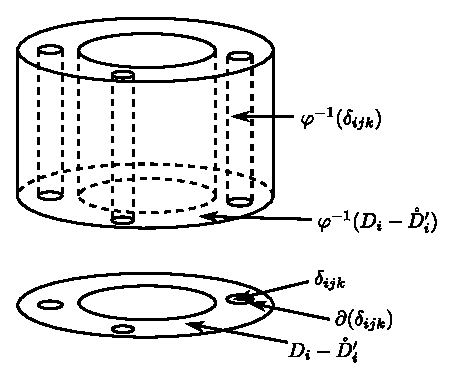
\includegraphics{fig15-3.eps}
\end{figure}
\end{proof}
We prove\pageoriginale

\begin{lemma}\label{art15-lem3.5}
$h^{q_1}$ induces a quasi-unipotent automorphism of $H_* (V_1)$ and of $H_* (\partial \delta_{1jk})$.

Actually this lemma is a consequence of 
\end{lemma}

\begin{lemma}\label{art15-lem3.6}
Let $\varphi: X \to Y$ be a smooth fibration of a smooth manifold $X$ onto a relatively compact manifold $Y$ and $\Psi: Y \to Y$ a mapping such that $\Psi^q = IdY$ and $h: X \to X$ such that we have the commutative diagram:
\[
\xymatrix@R=1.2cm{
X \ar[r]^{h} \ar[d]_\varphi & X \ar[d]^\varphi\\
Y \ar[r]^\Psi & Y 
}
\]
Suppose that the restriction of $h^q$ to $\varphi^{-1} (x)$ for any $x \in Y$ induces a quasi-unipotent automorphism of $H_* (\varphi^{-1} (x))$, then $h$ induces a quasi-unipotent automorphism of $H_* (X)$.
\end{lemma}

\begin{proof}
Considering $\Psi^q$ and $h^q$ instead of $\Psi$ and $h$ we may suppose that $\psi=\Id Y$.

Then our result follows from an obvious spectral sequence reasoning or we can prove it by considering a covering $U_1, \ldots, U_s$ of $Y$ by contractible open sets such that $U_i \cap U_j$ are contractible. Then prove by induction that the restriction of $h$ to $\varphi^{-1} (U_1 \cup \ldots \cup U_i)$, $i = 1, \ldots, s$ induces a quasi-unipotent automorphism of $H_* (\varphi^{-1} (U_1 \cup \ldots \cup U_i))$.

Now we have the Mayer-Vietoris sequence
$$
\to \bigoplus\limits_{j,k} H_k (\partial \delta_{1jk}) \to \bigoplus\limits_{j,k} H_k (\delta_{1jk}) \oplus H_k(V_1) \to H_k (U_1) \to .
$$

The actions of $h^{q_1}$ on $\bigoplus\limits_{j,k} H_k (\partial \delta_{1jk})$ and $H_k(V_1)$ are quasi-unipotent because the points of $\partial \delta_{1jk}$ and $V_1$ are rolling points. Thus this comes from our hypothesis 2) in (\ref{art15-lem3.3}) and the Lemma (\ref{art15-lem3.6}).
\end{proof}

{\em Thus we have proved (\ref{art15-lem3.4}) when $i=1$.}

Let us\pageoriginale suppose we have proved (\ref{art15-lem3.4}) for $1 \leqslant i < i_0$. We shall prove it for $H_* (U_{i_0})$. Notice that:
\begin{equation*}
U_{i_0} = U'_{i_0-1} U \varphi^{-1} (D_{i_0} - \mathring{D}'_{i_0-1}). 
\tag{3.7}\label{art15-eq3.7}
\end{equation*}

As $U_{i_0-1} \subset U'_{i_0-1}$ is a homotopy equivalence, the action of $h$ on $H_* (U'_{i_0-1})$ is quasi-unipotent. From Lemma (\ref{art15-lem3.6}) and the hypothesis 2) of (\ref{art15-lem3.3}) we obtain that the action on $H_* (\varphi^{-1} (\partial D'_{i_0-1}))$ is quasi-unipotent. We obtain our result by using again the Mayer-Vietoris sequence coming from (\ref{art15-eq3.7}) if we prove that the action of $h$ on $H_* (\varphi^{-1} (D_{i_0} - \mathring{D}'_{i_0-1}))$ is quasi-unipotent.

Let $\Psi_{i_0jk}: \delta_{i_0 jk} \to \delta_{i_0jk}$ be a distinguished carrousel associated to the roll $\Psi_{i_0}$. From the inductive hypothesis $h^{q_{i_0}}$ induces a quasi-unipotent automorphism of $H_* (\varphi^{-1} (\delta_{i_0 jk}))$. The Lemma (\ref{art15-lem3.6}) applies to $\varphi^{-1} (D_{i_0} - (\mathring{D}'_{i_0-1} \bigcup\limits_{j,k} \delta_{i_0 jk}))$ which is a smooth fibration onto $D_{i_0} - D'_{i_0-1} \bigcup\limits_{j,k} \delta_{i_0 jk} $ by $\varphi$. Thus because of (\ref{art15-lem3.6}) and 2) of (\ref{art15-lem3.3})$h^{qi_0}$ induces a quasi-unipotent automorphism of $H_* (\varphi^{-1} (D_{i_0} - (D'_{i_0 -1} \bigcup\limits_{j,k} \delta_{i_0jk}))$. For the same reason (application of the Lemma (\ref{art15-lem3.6})), $h^{qi_0}$ induces a quasi-unipotent automorphism of $H_* (\varphi^{-1} (\bigcup\limits_{j,k} \partial \delta_{i_0 jk}))$. Using again the Mayer-Vietoris argument, $h^{qi_0}$, thus $h$ itself, induces a quasi-unipotent automorphism of $H_* (\varphi^{-1} (D_{i_0} - \mathring{D}'_{i_0-1}))$.

Now our Theorem (\ref{art15-thm3.3}) is proved as $U_k \subset X$ is a homotopy equivalence, as $D - \mathring{D}_k$ does not contain any critical values of $\varphi$.

\setcounter{lemma}{7}
\begin{corollary}[Monodromy theorem]\label{art15-coro3.8}
The local monodromy of $f$ at $x$ is quasi-unipotent.
\end{corollary}

\noindent
{\bf Conclusion.}
The preceding proof has explicited a filtration of $H_* (F)$ where $F$ is the Milnor fibration and $F' = F \cap \{z_1 = 0\}$:
$$
H_* (F') \subset H_* (U_1) \subset H_* (U_2) \subset \ldots \subset H_* (U_k) = H_* (F)
$$
which is invariant under the action of the local monodromy.

One can prove that 
$$
H_* (F,F') \cong \bigoplus\limits^k_{i=1} H_* (U_i, U_{i-1}) \text{ with } U_0 = F'.
$$

The\pageoriginale relative monodromy on $H_* (F,F')$ is then the direct sum of the actions of $h$ on $H_* (U_i, U'_{i-1})$. By excision it is clear that $H_* (\varphi^{-1} (D_i - \mathring{D}'_{i-1}), \varphi^{-1} (\partial D'_{i-1}))$ is isomorphic to $H_* (U_i, U'_{i-1})$.

Now in the case of complex hypersurfaces of $\bfC^{n+1}$, one can prove that $H_n (\varphi^{-1} (\delta_{ijk})) =0$. Using a Mayer-Vietoris type argument as in the proof of the Lemma (\ref{art15-lem3.6}) above, we obtain that the relative monodromy induces an automorphism of $H_n(U_i, U_{i-1})$ the eigen values of which are $p_i$-th power of the eigenvalues of the local monodromy of the restriction of $z_1$ to the hypersurface $f^{q_i} - z^{p_i}_1 =0$, where $p_i$ and $q_i$ are integers, $(p_i, q_i) =1 $ and $2\pi \dfrac{p_1}{q_1}$ is the rotation angle of the roll $\Psi_i$.

By a more precise study of this geometry this should lead to an exact knowledge of the eigenvalues of the local monodromy by induction on the dimension. As it is seen the rotation angles $2\pi \dfrac{p_i}{q_i}$ interferes in this study. We want to point out that the interest of these $\dfrac{p_i}{q_i}$ have been arisen algebraically by B. Teissier in \cite{art15-key12} and \cite{art15-key13} in the case when $f=0$ is a complex hypersurface with isolated singularity. In \cite{art15-key10}, M. Merle has computed these numbers in terms of Puiseux exponents of the curve when $n=1$.

In fact it seems that one can likely study the Gauss-Manin connection of the singularity of $f$ at $x$ by using this geometry. This should lead to a relative Gauss-Manin connection. One expects a knowledge about the link between the roots of the $b$-polynomial (Bernstein polynomial) of $f$ and the eigenvalues of its local monodromy at $x$ as it has been done by B. Malgrange in \cite{art15-key9}. This should give another proof of the rationality of the roots of the $b$-polynomial  which does not use the resolution of the singularities of $f$ (cf. \cite{art15-key4}).

\begin{thebibliography}{99}
\bibitem{art15-key1} H. Clemens, P. Griffiths, N. Katz and alii: {\em Seminar on degeneration of algebraic varieties,} Preprint, Princeton (1969).

\bibitem{art15-key2} A. Grothendieck:\pageoriginale S.G.A. VII t. 1, {\em Springer Lecture Notes,} 288.

\bibitem{art15-key3} H. Hamm: Lokale topologische Eigenschaften komplexer R\"{a}ume, {\em Math. Ann.}  191, 235-252 (1971).

\bibitem{art15-key4} M. Kashiwara: $B$-functions and holomorphic systems, {\em Inv. Math.} (1976).

\bibitem{art15-key5} A. Landman: On the Picard-Lefchetz transformation for algebraic manifolds acquiring general singularities, {\em Trans. Amer. Math. Soc. } 181 (1973), 89-126.
 

\bibitem{art15-key6} L$\hat{\text{e}}$ D$\tilde{\text{u}}$ng Tr\'ang: Remarks on relative monodromy, {\em Proc. of Nordic Summer School at Oslo} (1976).

\bibitem{art15-key7} L$\hat{\text{e}}$ D$\tilde{\text{u}}$ng Tr\'ang: La monodromie n'a pas de points fixes, {\em J. of Fac. Sc., Univ. Tokyo, Sec.} 1A, vol. 22 (1975), 409-427.

\bibitem{art15-key8} L$\hat{\text{e}}$ D$\tilde{\text{u}}$ng Tr\'ang: Calcul des cycles \'evanouissants des hypersurfaces complexes, {\em Ann. Inst. Fourier} (1973).

\bibitem{art15-key9} B. Malgrange: Sur les polyn\`omes de I.N. Bernstein, {\em Uspechi Math. Nauk } 29 (4) (1974), 81-88.

\bibitem{art15-key10} M. Merle: Invariants polaires de courbes planes, to be published in {\em Inv. Math.}


\bibitem{art15-key11} J. Milnor: Singular points of complex hypersurfaces, {\em Ann. Math. Stud.} 61, Princeton. 

\bibitem{art15-key12} B. Teissier: Invariants  polaires des hypersurfaces, to be published in {\em Inv. Math.}

\bibitem{art15-key13} B. Teissier: The hunting of invariants in the geometry of discriminants, {\em Proc. of Nordic Summer School at Oslo } (1976).

\end{thebibliography}
